\documentclass{article}

\usepackage[preprint]{neurips_2021}

\usepackage[
backend=biber,
style=alphabetic,
sorting=ynt
]{biblatex}

% to compile a preprint version, e.g., for submission to arXiv, add the
% [preprint] option:
%     \usepackage[preprint]{neurips_2021}

% to compile a camera-ready version, add the [final] option, e.g.:
%     \usepackage[final]{neurips_2021}

% to avoid loading the natbib package, add option nonatbib:
%    \usepackage[nonatbib]{neurips_2021}

\usepackage[utf8]{inputenc} % allow utf-8 input
\usepackage[T1]{fontenc}    % use 8-bit T1 fonts
\usepackage{hyperref}       % hyperlinks
\usepackage{url}            % simple URL typesettinge
\usepackage{booktabs}       % professional-quality tables
\usepackage{amsfonts}       % blackboard math symbols
\usepackage{nicefrac}       % compact symbols for 1/2, etc.
\usepackage{microtype}      % microtypography
\usepackage{xcolor}         % colors
\usepackage{algpseudocode}
\usepackage{graphicx}

\addbibresource{main.bib}

\title{Applying Bounding Box Detection on the Invasive COTS Starfish to Protect Coral Reefs}

\author{
    Luke Wood \\
    \texttt{l2wood@ucsd.edu} \\
    \And 
    Harsh Kishorsingh Thakur \\
    \texttt{hthakur@ucsd.edu} \\
    \And 
    Sandra Villamar \\
  \texttt{svillama@ucsd.edu} \\
}

\begin{document}

\maketitle

\begin{abstract}
Due to the diminishing population of the Charonia Tritonis sea snail, the population of Crown-of-Thorns starfish (COTS) has grown rapidly across all regions of the Great Barrier Reef. COTS eat coral which ultimately destroys coral reef ecosystems. The species pose a massive existential threat to the Great Barrier Reef. The traditional way of detecting COTS is the “Manta Tow” method, in which a diver records sightings while being physically towed behind a boat. This method is clearly inefficient, unreliable, and costly. In order to automate this process, our team has produced a deep learning bounding box detection model to detect COTS from the reef images.

\hyperlink{https://github.com/lukewood/reef-net}{The code for all of our experiments is available in our GitHub repo as: https://github.com/lukewood/reef-net}
\end{abstract}

\section{Introduction}
Australia’s Great Barrier Reef is the world’s largest coral reef system, containing a unique range of ecological communities, habitats, and species. Over half a billion people rely on coral reefs for food, income, and protection against storms and erosion along coastlines \cite{coralreefecosystems}. Unfortunately, the Great Barrier Reef is under threat in part due to the overpopulation of coral-eating Crown-of-Thorns starfish (COTS). One of the largest sea stars in the world, COTS can have up to 21 arms covered in poisonous spines. They are an integral part of the reef ecosystem, but their population exploded when their chief predators, the Charonia Tritonis sea snail, were excessively hunted by shell collectors. This has created an imbalance in the ecosystem.

Furthermore, recent increases in ocean temperatures due to human activities have caused massive coral bleaching throughout the Great Barrier Reef. Corals can survive a bleaching event, but they are under more stress and are subject to mortality. Millions of corals have already died, but we have the ability to slow down this decay if we control other factors that contribute to the deterioration of the Great Barrier Reef. Hopefully, by controlling the outbreak of COTS, the Great Barrier Reef will have the opportunity to recover. Due to the overpopulation of COTS, a large-scale intervention program was established to control COTS outbreaks to ecologically sustainable levels. The traditional way of surveying COTS is the “Manta Tow” method, where divers are towed along the reef, pausing ever so often to dive down and record how many COTS are visible. With such a large ocean bed, this method is clearly inefficient, unreliable, and costly. In order to improve the efficiency and scale of identifying COTS outbreaks, the Great Barrier Reef Foundation has collected thousands of reef images taken with underwater cameras and published this data set \cite{cots_dataset} to a Kaggle competition, in hopes of adopting a new detection method through AI technology. The Kaggle data set consists of 23k images, around 4k of which contain at least one COTS.

We use a RetinaNet to perform object detection in an attempt to localize COTS. A sufficiently performant model will obsolete the "Manta Tow" method, greatly improving the efficiency and reducing the cost of COTS detection.

Our contributions are as follows:
\begin{enumerate}
    \item a data loader to produce a TensorFlow data set from the raw data
    \item basic preprocessing and image augmentation utilities
    \item ground truth and detection visualization tools
    \item a custom Keras implementation of the RetinaNet algorithm
    \item robust metric tracking, all in the TensorFlow graph using KerasCV's COCO metrics implementation \cite{wood2022kerascv}
    \item a Keras callback to visualize results each training epoch
    \item a custom tool to produce train-test splits for the TensorFlow Great Barrier Reef data set
\end{enumerate}

\section{Related Works}
There exist countless publications on deep learning based works on bounding box detection methods.
The MSCOCO challenge popularized the problem \cite{coco}.
Alongside the MSCOCO object detection challenge, the data set publishers also published a set of evaluation metrics: Mean Average Precision and Recall \cite{coco}.
Our work is based on RetinaNet proposed by Li et al \cite{retinanet}.
The loss is also proposed by Li et al in the same work.

Other modern bounding box detection models include the two stage Faster-RCNN \cite{rcnn}, YOLOv5 \cite{yolov4} and YOLOx \cite{yolox}.
Other similar tasks include \textit{Keypoint Detection} and \textit{Semantic segmentation} \cite{9356353}.

\section{Problem Formulation}
In this project we are trying to achieve the task of object detection. 
Object detection consists of two sub-tasks: 

\textbf{Object Localization}: locating one or more target objects within the image.
\begin{itemize}
    \item \textit{Input}: an image with zero or more objects
    \item \textit{Output}: zero or more bounding boxes represented by four number tuples.  These are often represented as (x, y, width, height) coordinates of the bounding boxes.
\end{itemize}

\textbf{Object Classification}: classification of the objects inside of each predicted bounding box.
\begin{itemize}
    \item \textit{Input}: section of the image obtained from the corresponding bounding box
    \item \textit{Output}: class to which the objects in the predicted bounding boxed belongs to
\end{itemize}

Object detection is achieved by performing both of these tasks simultaneously.
In short, the task of object detection can be defined as transforming an input image to one or more bounding boxes and accompanying class labels.
In our case, the only valid class label is COTS starfish.

In mathematical terms the goal of object detection is as follows for each image:

\textbf{Object Localization:}

Define $X=image$ and $y=bounding boxes$. \\
Then $y\_pred=\Theta(X)$, i.e. a function of $X$ consisting of: \\
\begin{itemize}
    \item  $box\_pred$ = $y\_pred[:, :4]$, the coordinates of the bounding boxes \\
    \item $class\_pred = y\_pred[:, 5]$, the class label \\
\end{itemize}

We want to find $\Theta$ such that: \\

$\Theta\ = argmin_{\Theta}\{MSE(box\_pred, y[:, :4]) + CrossEntropy(class\_pred, y[:, 5])\}$ \\

The goal of bounding box detection is to achieve a parameterization of $\Theta$ to satisfy these conditions.

% Look I made you something:
%   ,--,    .---.    .-. .-.  .--.  ,---.    .---. .-. .-. 
% .' .'    / .-. )   | | | | / /\ \ | .-.\  ( .-._)| | | | 
% |  |  __ | | |(_)  | `-' |/ /__\ \| `-'/ (_) \   | `-' | 
% \  \ ( _)| | | |   | .-. ||  __  ||   (  _  \ \  | .-. | 
%  \  `-) )\ `-' /   | | |)|| |  |)|| |\ \( `-'  ) | | |)| 
%  )\____/  )---'    /(  (_)|_|  (_)|_| \)\`----'  /(  (_) 
% (__)     (_)      (__)                (__)      (__)     


\section{Method/Approach}
We propose a bounding box prediction model to predict the presence and position of COTS along with a confidence score for each identified starfish. This is done using a RetinaNet model implemented in Keras that we refer to as ReefNet. Despite being a one stage object detection msodel, RetinaNet is the current state of the art object detection model, achieving the highest mean average precision (MaP) of any model on the \textit{MS COCO} data set \cite{retinanet}\cite{coco}. 

Our repository consists of a data loader, basic augmentation pipeline, RetinaNet model, visualization callbacks, and an evaluation pipeline. Figure \ref{fig:approach_overview} provides an overview of the logical flow of our approach.

\begin{figure}
    \centering
    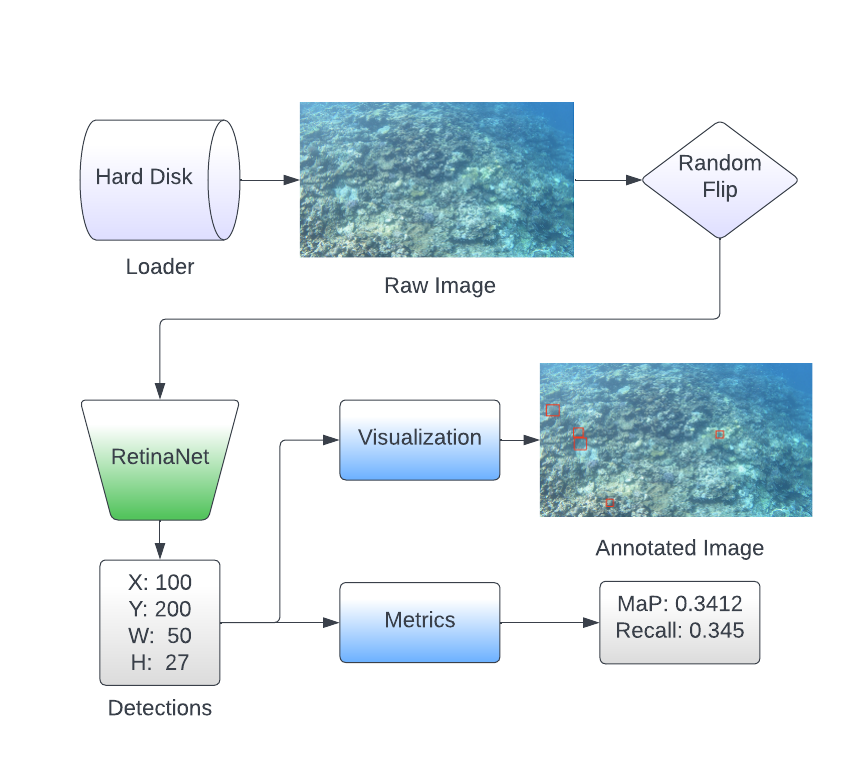
\includegraphics[width=\textwidth]{overview.png}
    \caption{Overview of our Approach}
    \label{fig:approach_overview}
\end{figure}

\subsection{Data and Preprocessing}
The raw data set consists of 23,501 underwater images taken at various times and locations around the Great Barrier Reef, as well as metadata for the images which include the associated video and sequence IDs, along with the bounding box coordinates of any starfish detections. Figure \ref{fig:sample_data} displays two samples from the data set overlaid with the annotated bounding boxes, each identifying a starfish.
We split the data set into 80\% training, 10\% validation, and 10\% testing with about 20K examples for training and 2K examples for validation and testing.  

In order to apply augmentations to our data set, we first convert the bounding box format from (x-coordinate of upper left corner, y-coordinate of upper left corner, width, height) in pixels to (x-coordinate of upper left corner, y-coordinate of upper left corner, x-coordinate of lower right corner, y-coordinate of lower right corner) in relative units to image shape. Next, we apply two types of augmentations; The first horizontally flips the image and corresponding bounding boxes with a 50\% chance. The second resizes and pads the image to a given shape, using a random jitter for the smallest dimension. Lastly, we convert the format of the bounding boxes to (x-coordinate of center, y-coordinate of center, width, height) in relative units to image shape.

\begin{figure}[!ht]
    \begin{minipage}{0.48\textwidth}
    \centering
    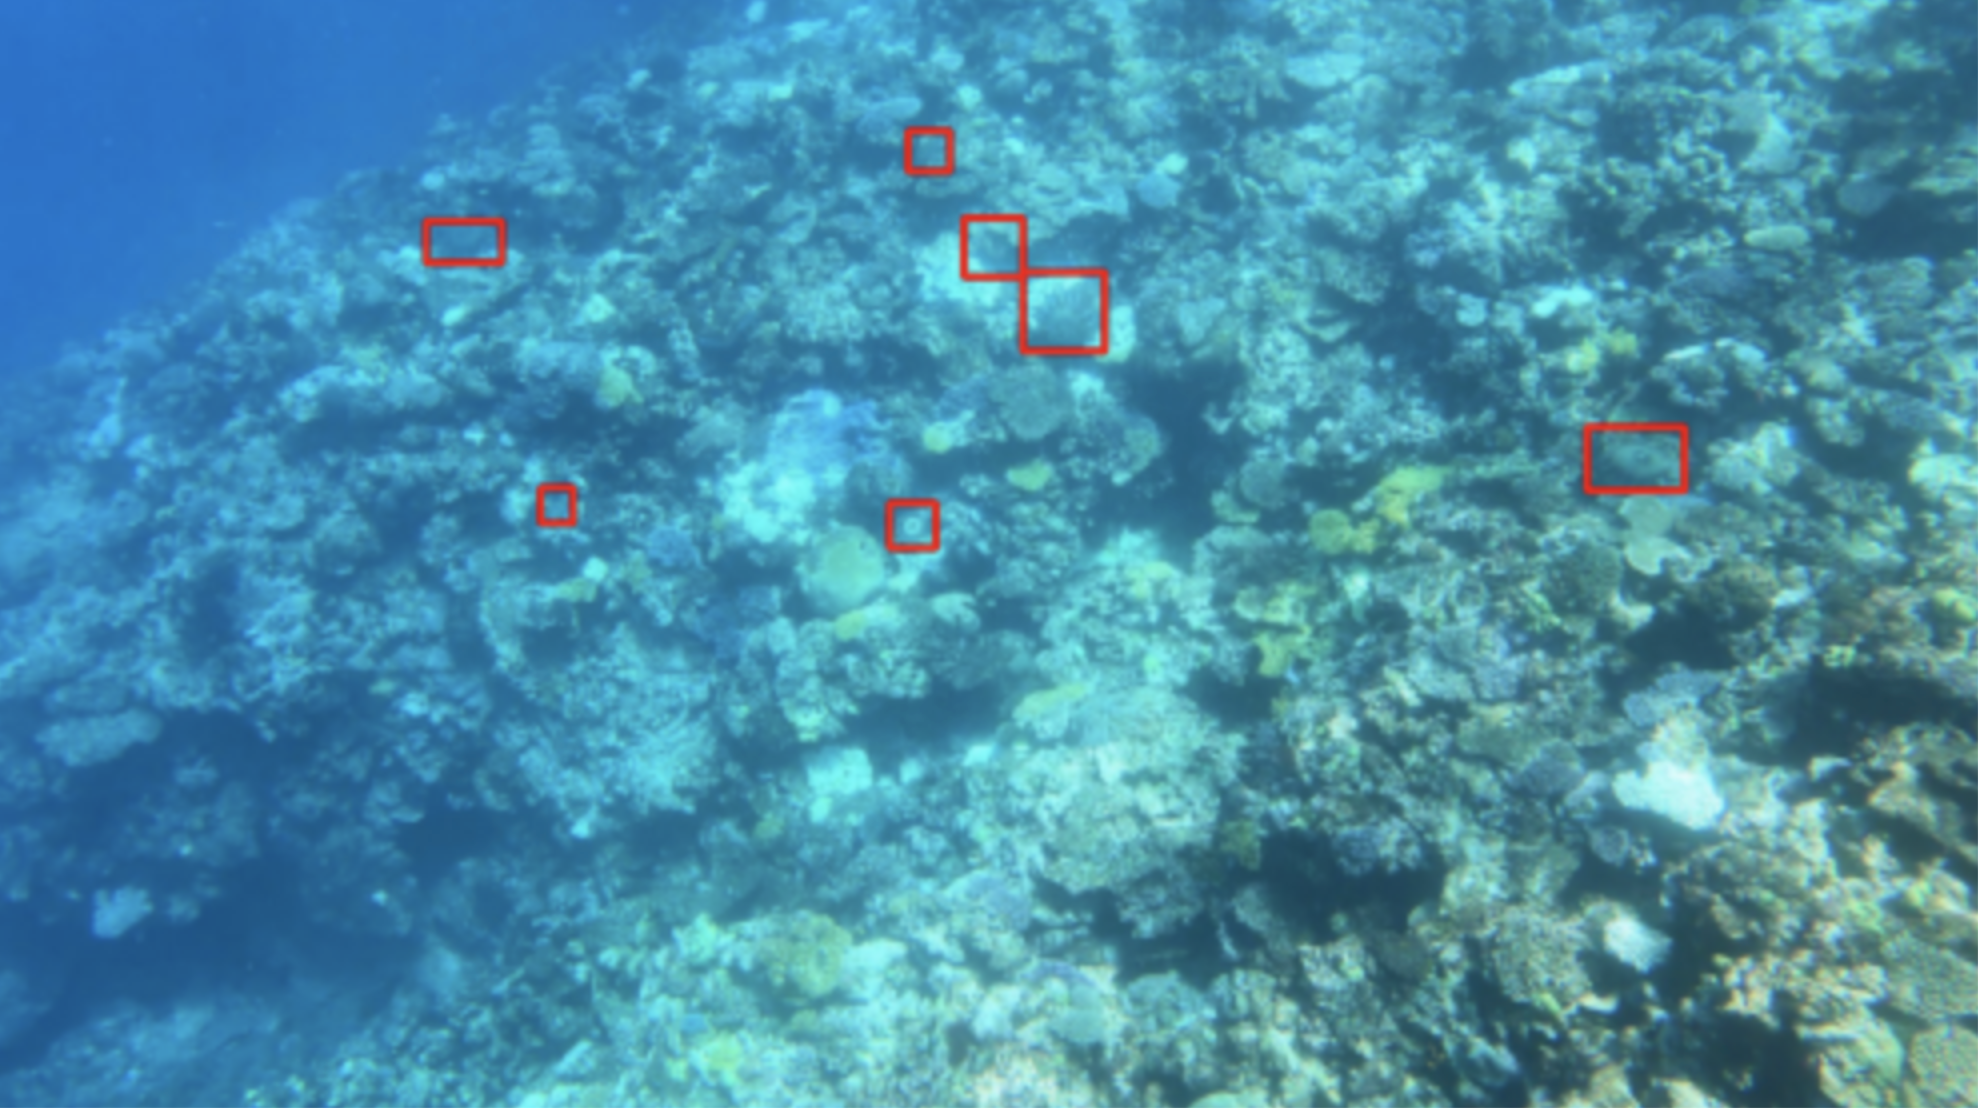
\includegraphics[width=\textwidth]{demo_image.png}
    \end{minipage}
    \begin{minipage}{0.48\textwidth}
    \centering
    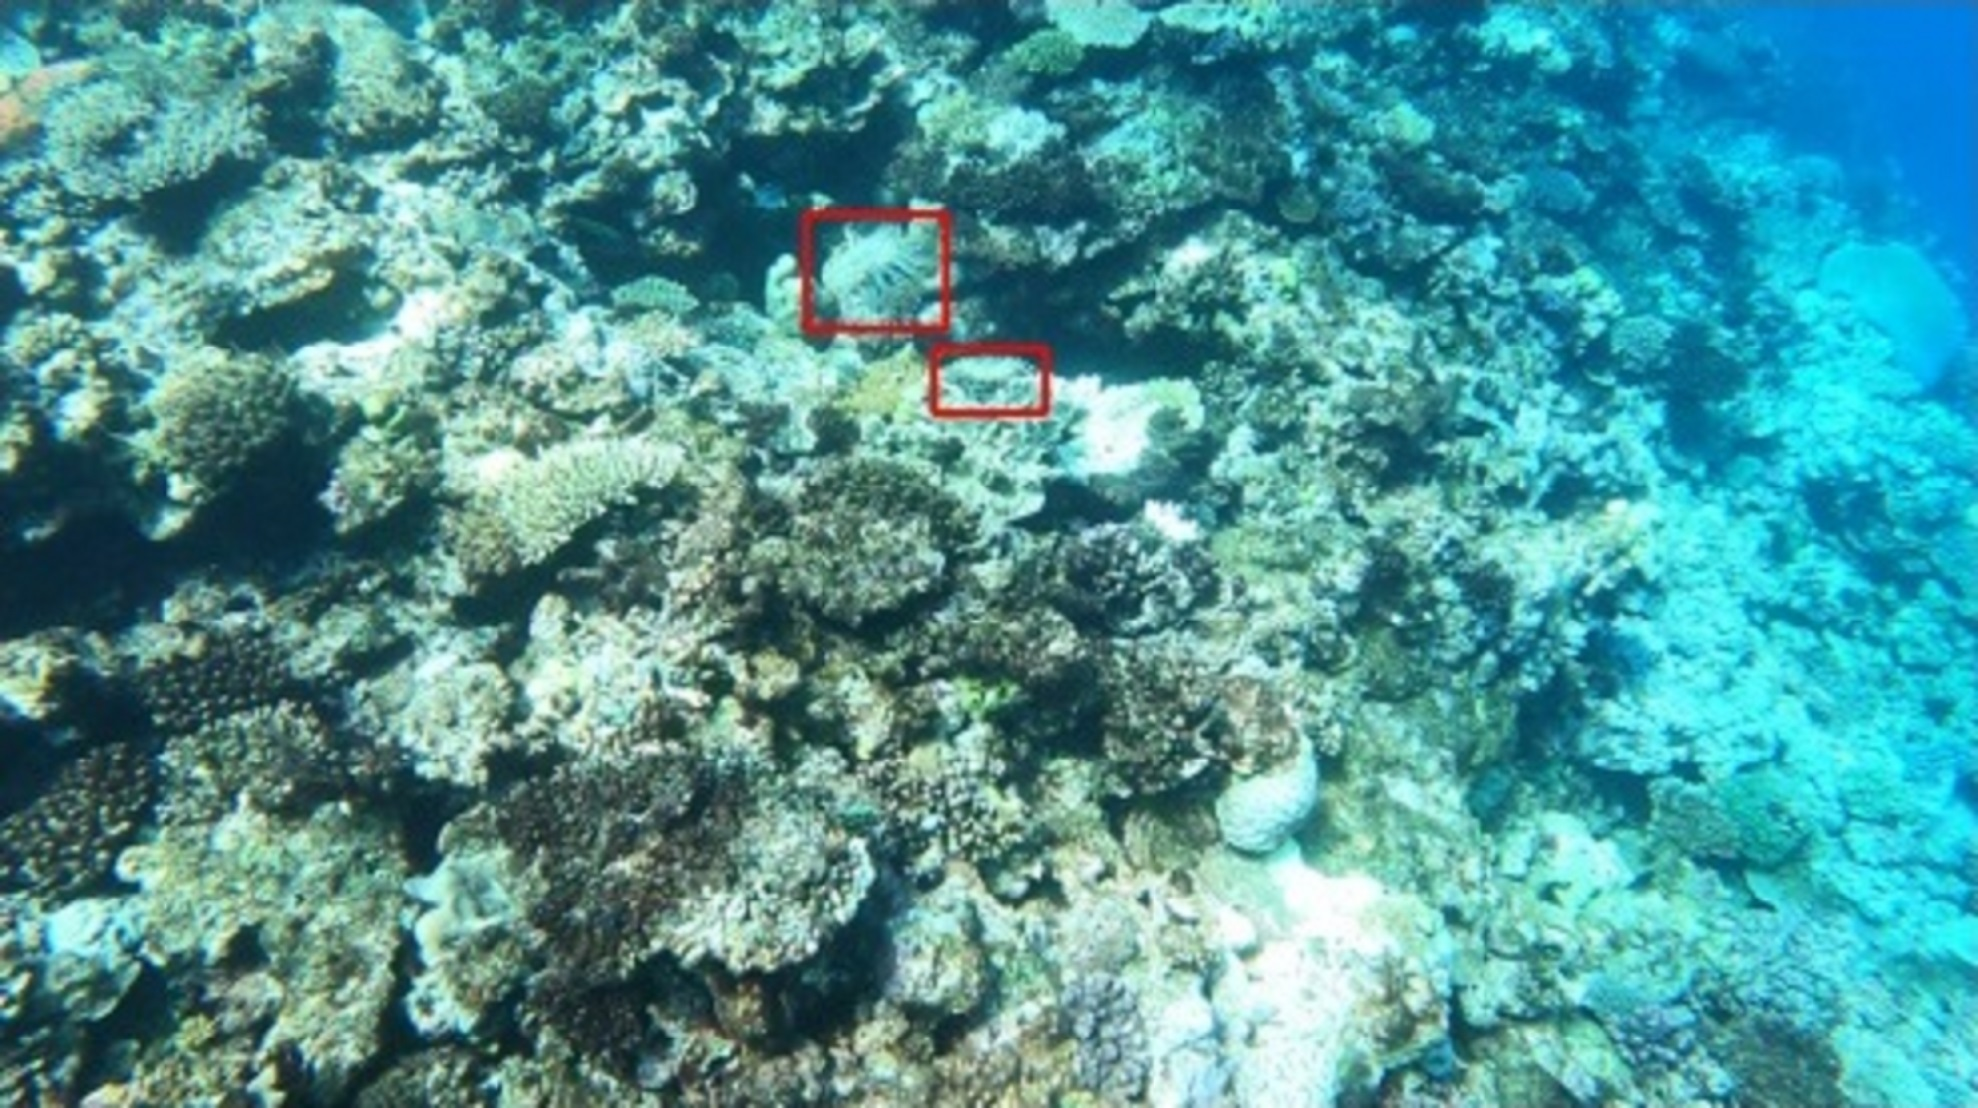
\includegraphics[width=\textwidth]{demo_image_2.jpg}
    \end{minipage}
    \caption{Sample Detection Image With Overlaid Bounding Boxes}
    \label{fig:sample_data}
\end{figure}


\subsection{Model}
ReefNet is an implementation of the RetinaNet object detection architecture.
Although RetinaNet is a single-stage object detection model, it still manages to obtain exceptional MaP and recall by leveraging a Feature Pyramid along with the focal loss function \cite{retinanet}.
This allows us to perform real-time inference while achieving high performance metrics.
Our model in particular uses a ResNet50 encoder in the Feature Pyramid \cite{feature_pyramid}\cite{resnet}.

One key component of object detection networks are anchor boxes: fixed-size boxes that are used to predict bounding boxes.

Anchor boxes are used in RetinaNet in the following way:
First, the model predicts whether or not a given anchor box contains an object. 
Following this, the model predicts the difference between the object center, width, and height from the anchor box.

During training, ground truth labels are transformed into RetinaNet prediction targets.
The model generates 202,554 anchor boxes with varying sizes and corresponding aspect ratios for each training image.
This is done using an AnchorBox generator, which produces 9 anchor boxes for each sampled location feature in a given feature map.
The generator samples locations in strides of varying sizes, from 9 pixels for small boxes to 256 pixels for large boxes.
The anchor boxes are also generated with areas ranging from $1024\: px^2$ to $262k\: px^2$.
The generated bounding boxes are then assigned to either the background class (an ignore class) or the COTS class, depending on how high their intersection over union (IoU) ratio is with the ground truth bounding box.
Finally, these generated boxes are used to produce box prediction and classification targets. 
This process matches the label encoding procedure used in the original RetinaNet implementation.
These targets are then used in training alongside the RetinaNet loss, fully described in Section \ref{sec:loss}.

\subsection{Loss}
\label{sec:loss}

RetinaNet is typically trained using two loss functions: a classification and a box loss.  The combination of these two losses is colloquially referred to as FocalLoss.  FocalLoss applies a modulating term to standard cross entropy in order to focus learning on hard misclassified examples.
In the case of ReeNet, the COTS examples are considered the hard examples .
Focal loss is useful for cases where there is a class imbalance and is hence particularly common in object detection, as most of the image belongs to the background class and only a few pixels in the image contain the object of interest.

The classification loss is used to identify whether the predicted bounding box belongs to the background or contains a starfish. As we are only detecting starfish, any box not containing a starfish, i.e. classified as background, is only considered in the classification loss.

Additionally, we have the box loss, which is applied to all bounding boxes that should have been classified correctly as starfish.
This loss allows the model to produce more accurate predictions for each detected COT starfish. 
We implement box loss with smooth L1 loss, which acts as L1-loss when the absolute value of the argument is large, generating steady gradients, and acts as L2-loss when the absolute value of the argument is close to zero, causing less oscillations during updates. 

\subsection{Training}
% INCLUDE: hyperparameter being used & loss/training curves
% we ran two experiments.
% 1.) Adam optimizer, learning_rate=0.001, beta_1=0.9, beta_2=0.999, epsilon=1e-7
% 2.) SGD optimizer, custom learning rate schedule
% the learning rate schedule is defined as follows:
% learning_rates = [[2.5e-06, 0.000625, 0.00125, 0.0025, 0.00025, 2.5e-05]]
% learning_rate_boundaries=[125, 250, 500, 240000, 360000] 

In our experiments we trained two models.  These models are trained using identical procedures, with the exception of optimizer choice.  One model is trained using the Adam optimizer with a $learning\_rate=0.001$, $\beta_1=0.9$ value of 0.9, $\beta_2=0.999$ value of 0.999, and an $\epsilon=1^{-10}$.  The SGD optimizer is configured with $momentum=0.9$, a custom learning rate schedule with learning rates [2.5e-06, 0.000625, 0.00125, 0.0025, 0.00025, 2.5e-05], and learning rate boundaries set at [125, 250, 500, 240000, 360000] steps respectively.

Both models are trained with a batch size of 2 due to the high memory requirements of the encoded labels.  Our models are trained to convergence when possible, which typically occurs in under 100 epochs.
ReefNets are trained only on images with at least one COT starfish present.
Images are also fed through the data augmentation pipeline which performs a random flip with a 50\% probability.

During training, the models generate predictions.  These predictions are used to evaluate the MSCOCO evaluation metrics: MaP and Recall.  These predictions are also used to generate visualizations, which are ultimately merged into a video that showcases the training process of the ReefNet.
For real time loss and metric monitoring our metrics are exported to both TensorBoard and Weights and Biases.
An example video is available in \hyperlink{https://github.com/lukewood/reef-net}{the ReefNet GitHub repository}.

\section{Results}
The model trained using Adam performs extremely poorly.  Figure \ref{fig:loss_comparison} shows that the loss never stabilized, and also converged at an extremely high value.  In addition to the loss of the Adam trained model having extremely high variance throughout the entirety of training, the loss also failed to converge.  The same pattern is present in the validation loss.

Compare this to the SGD trained model, shown by the yellow line in figure \ref{fig:loss_comparison}.  The SGD trained model achieves a much more stable learning curve.  The SGD trained model is also able to converge on a significantly lower loss.  This pattern holds when examining the box loss, also shown in figure \ref{fig:loss_comparison}, as well as the classification loss.

During training, our custom Keras visualization callback performs model inference on a single image on each epoch end. 
Figure \ref{fig:sample_visualizations} shows the ground truth of one such image (left) as well as our models prediction at the final training epoch (right).
\href{https://github.com/lukewood/reef-net}{Our GitHub repository also contains a video showcasing predictions after each training epoch of the final SGD model}.

Figure \ref{fig:results_loss} shows that ReefNet successfully converges, while 
figure \ref{fig:metrics_eval} shows the results of both the MSCOCO Mean Average Precision and MSCOCO Recall evaluation metrics\cite{coco}.
Reefnet uses the KerasCV COCO metrics implementation\cite{wood2022kerascv}.
Our model quickly achieves a high Recall score, indicating that the model is able to consistently locate over 70\% starfish.
Unfortunately, ReefNet's Mean Average Precision score is significantly weaker.
The discrepancy between Recall and Mean Average Precision indicates that the model is likely performing too many false positive predictions.
Figure \ref{fig:sample_visualizations} shows that this is indeed the case, with the model having made several false positive predictions on the right hand side of the image.

\begin{figure}
    \begin{minipage}{0.48\textwidth}
        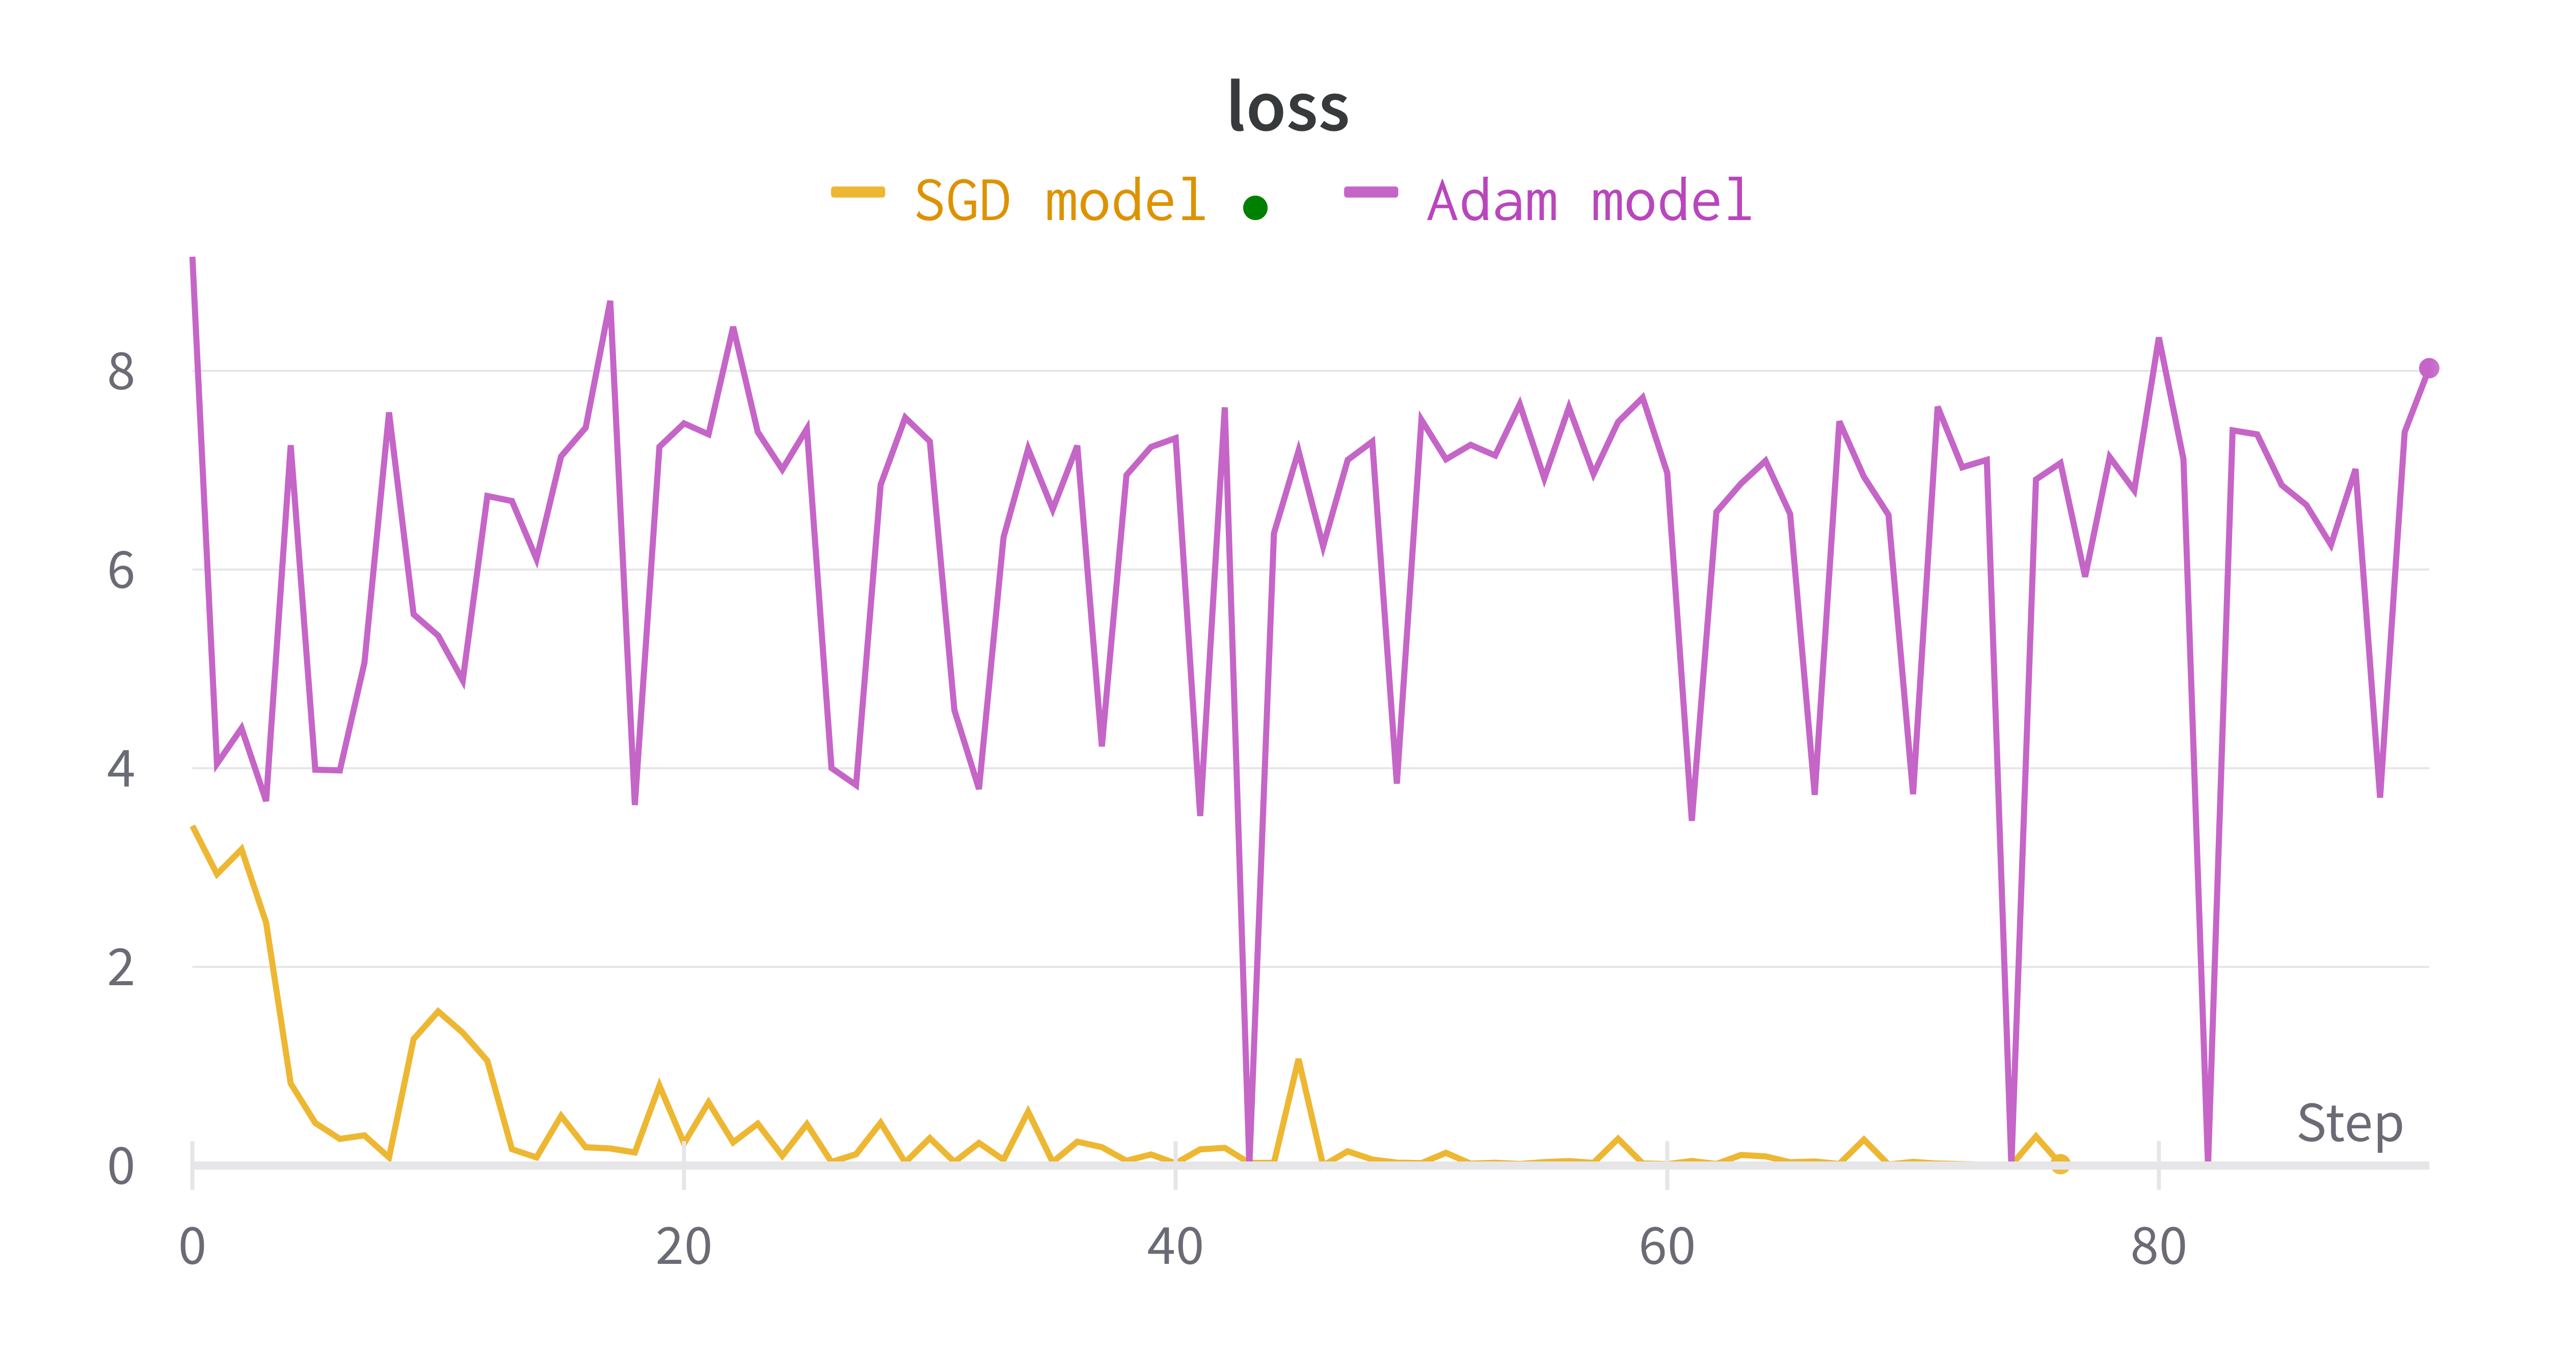
\includegraphics[width=\textwidth]{comparison_loss.png}
    \end{minipage}
    \begin{minipage}{0.48\textwidth}
        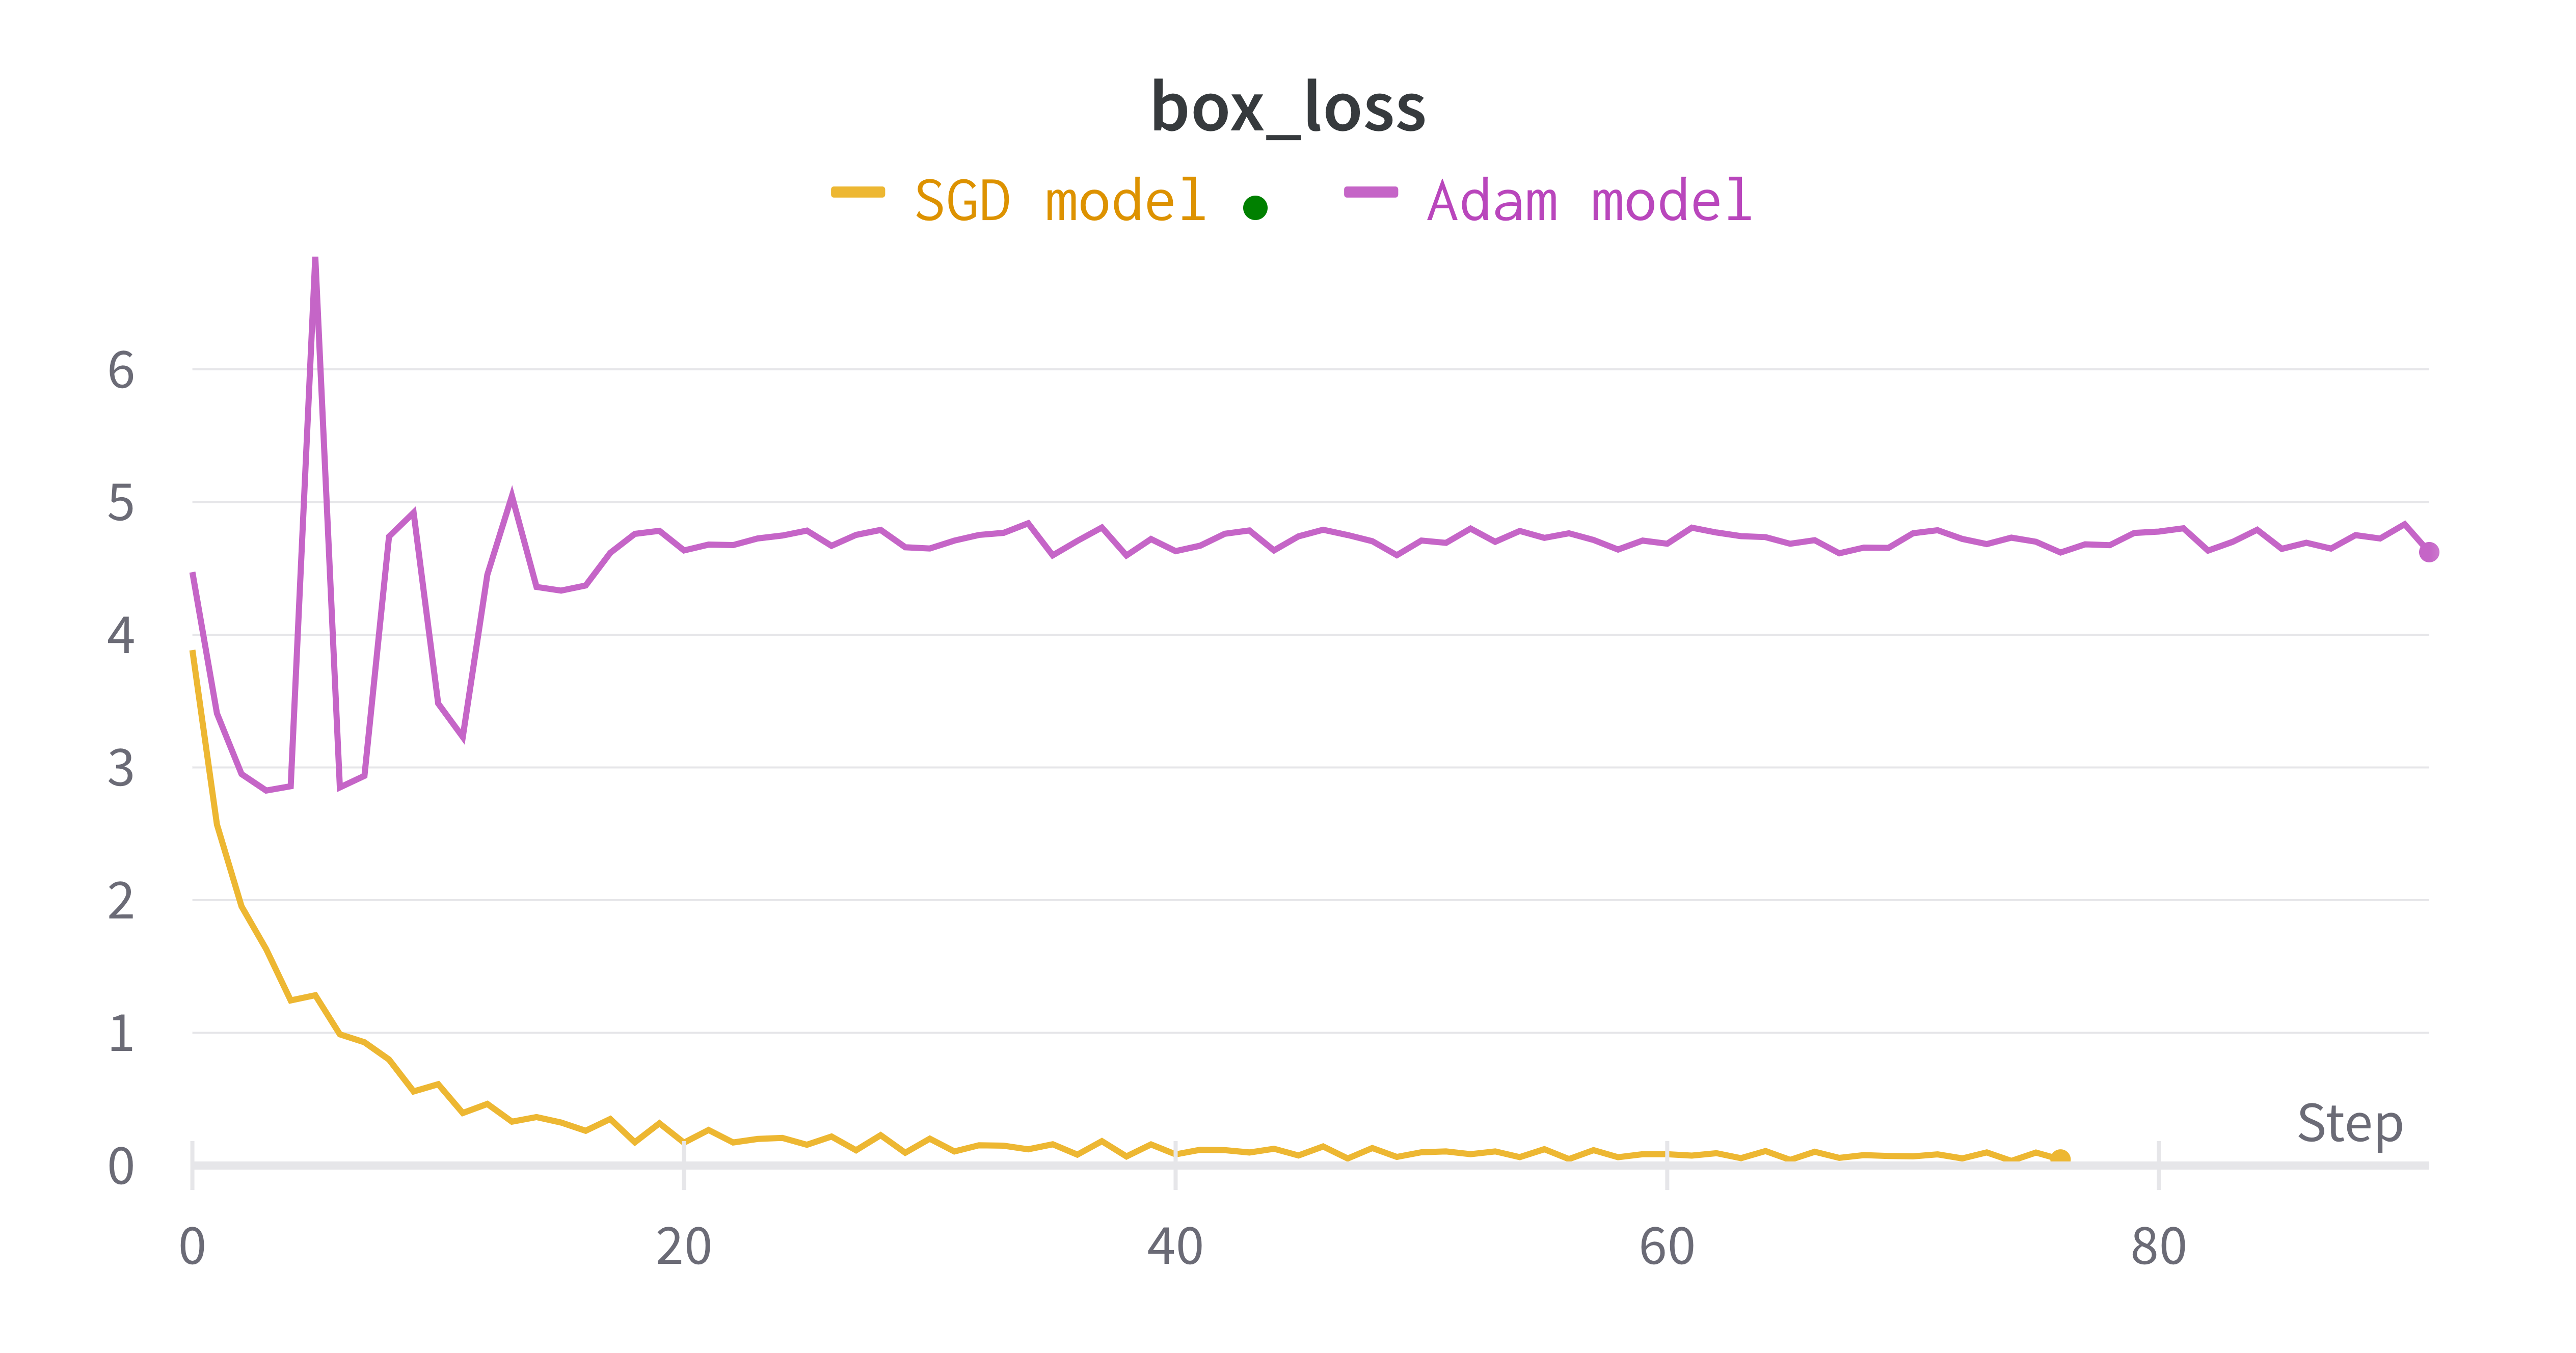
\includegraphics[width=\textwidth]{comparison_box_loss.png}
    \end{minipage}
    \caption{Loss Comparison of the SGD and Adam Trained Models}
    \label{fig:loss_comparison}
\end{figure}


\begin{figure}
    \begin{minipage}{0.48\textwidth}
        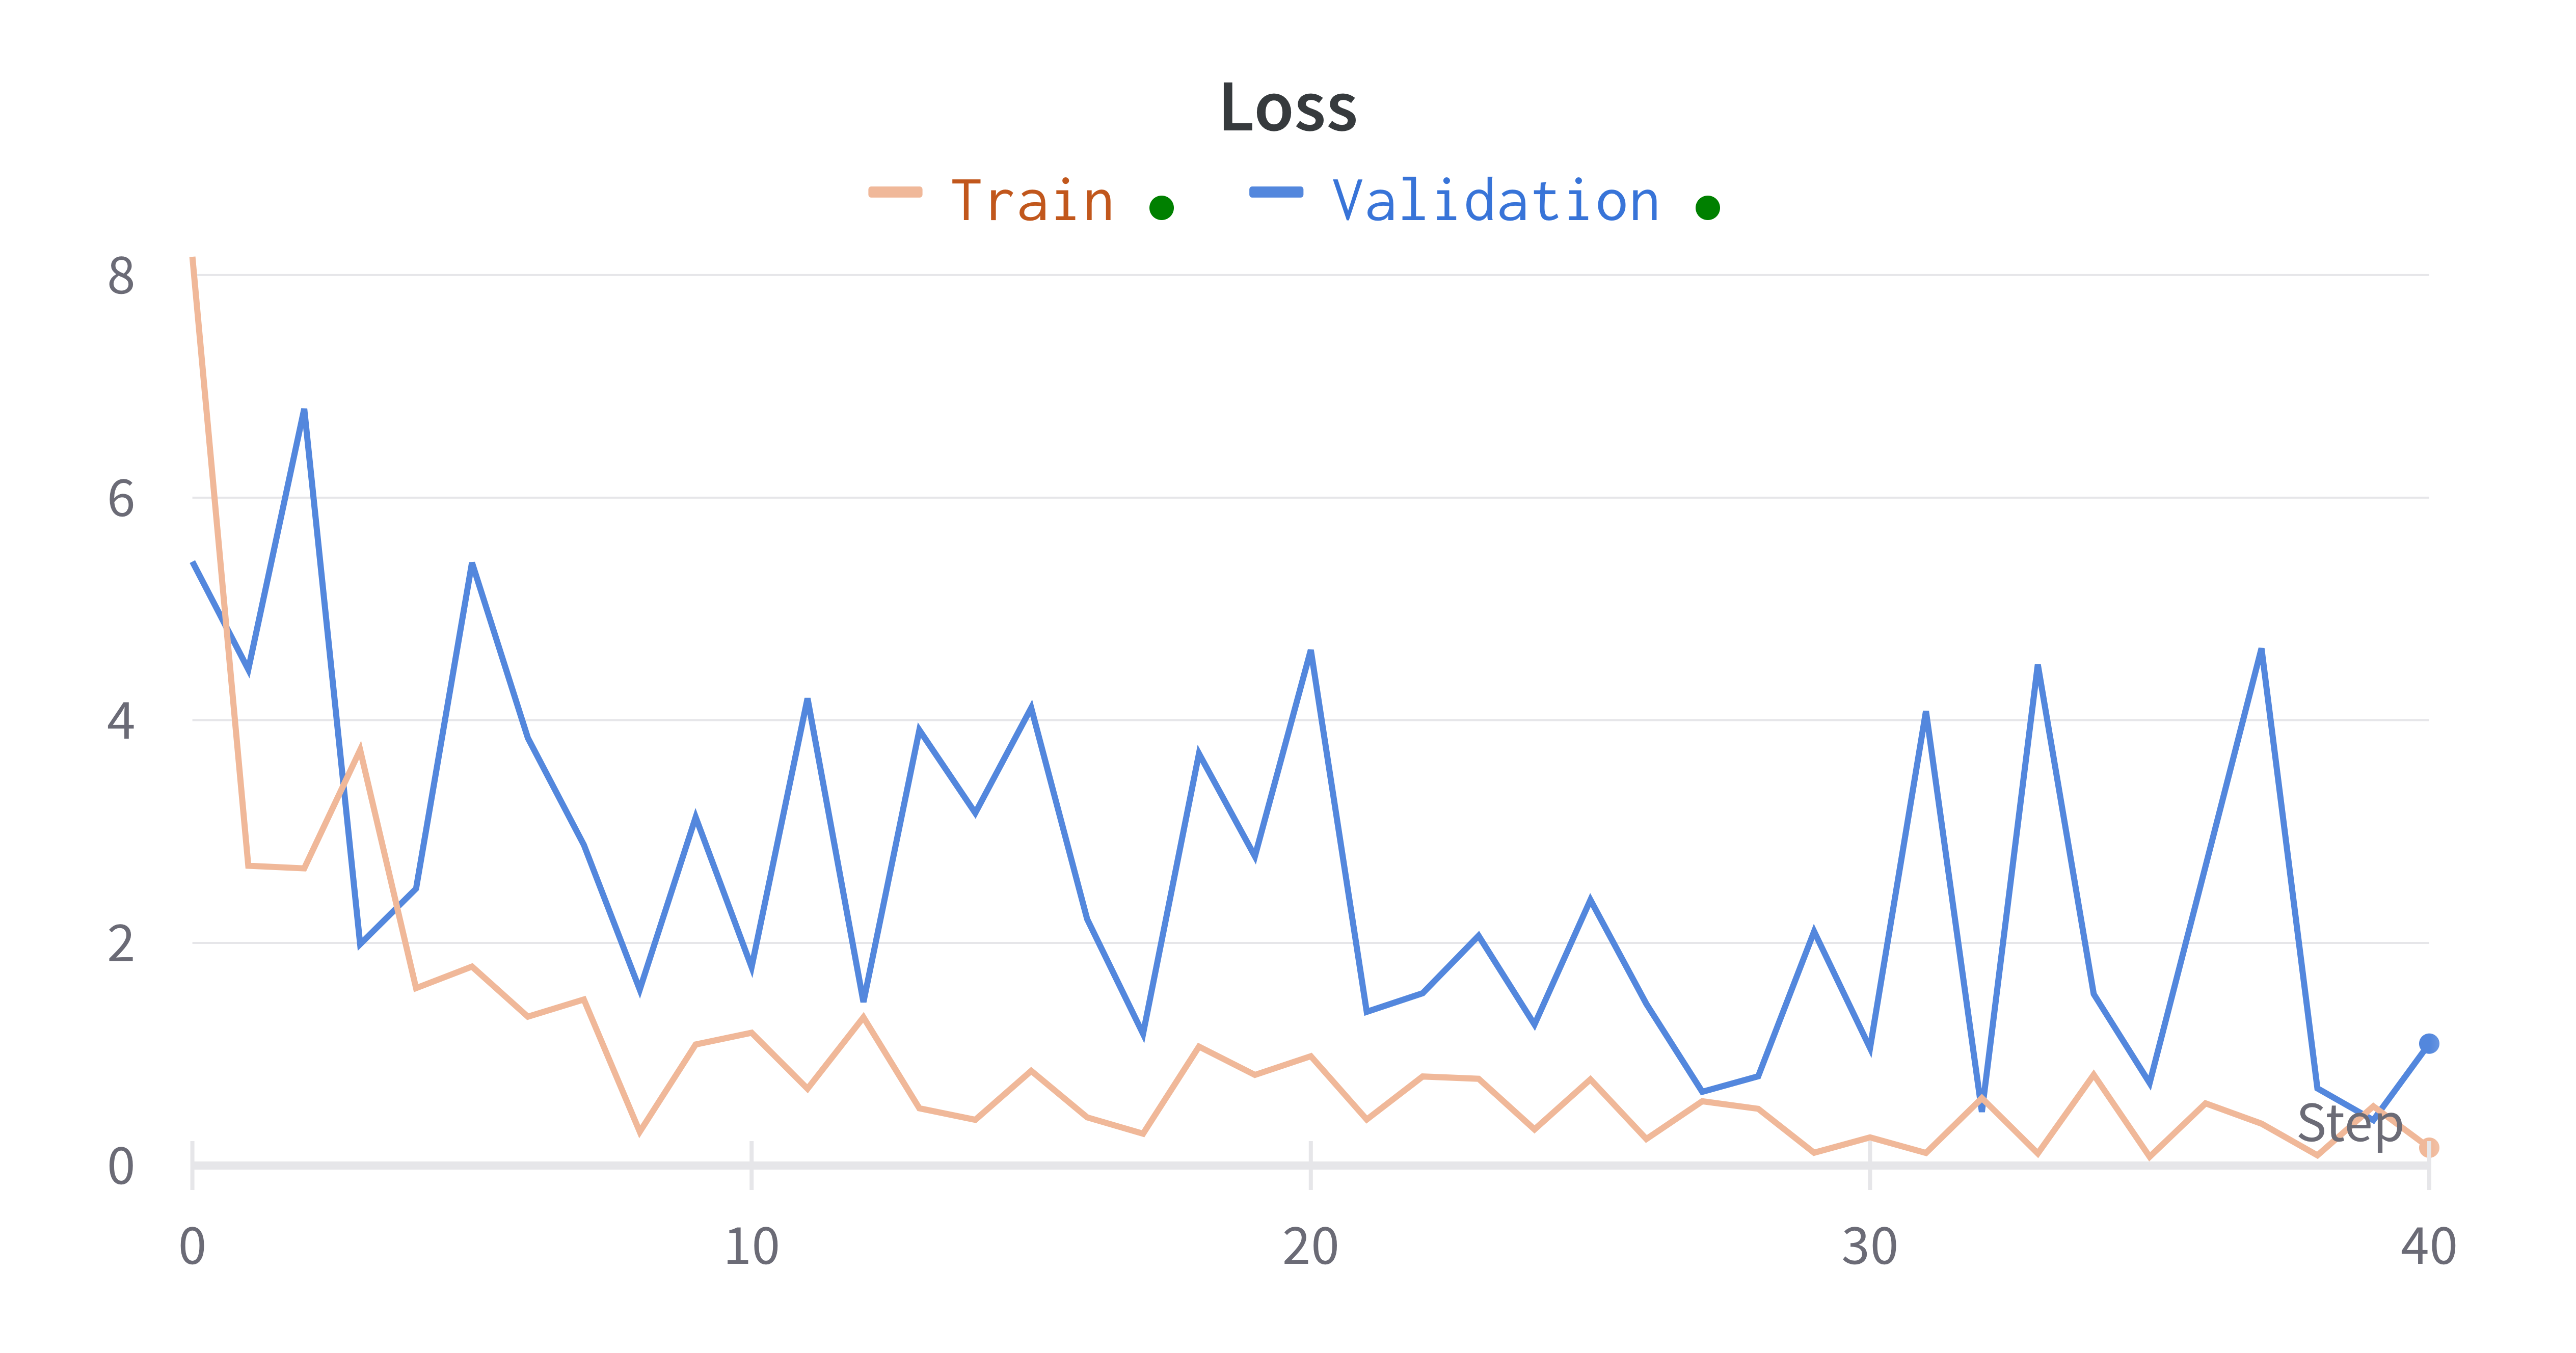
\includegraphics[width=\textwidth]{loss.png}
    \end{minipage}
    \begin{minipage}{0.48\textwidth}
        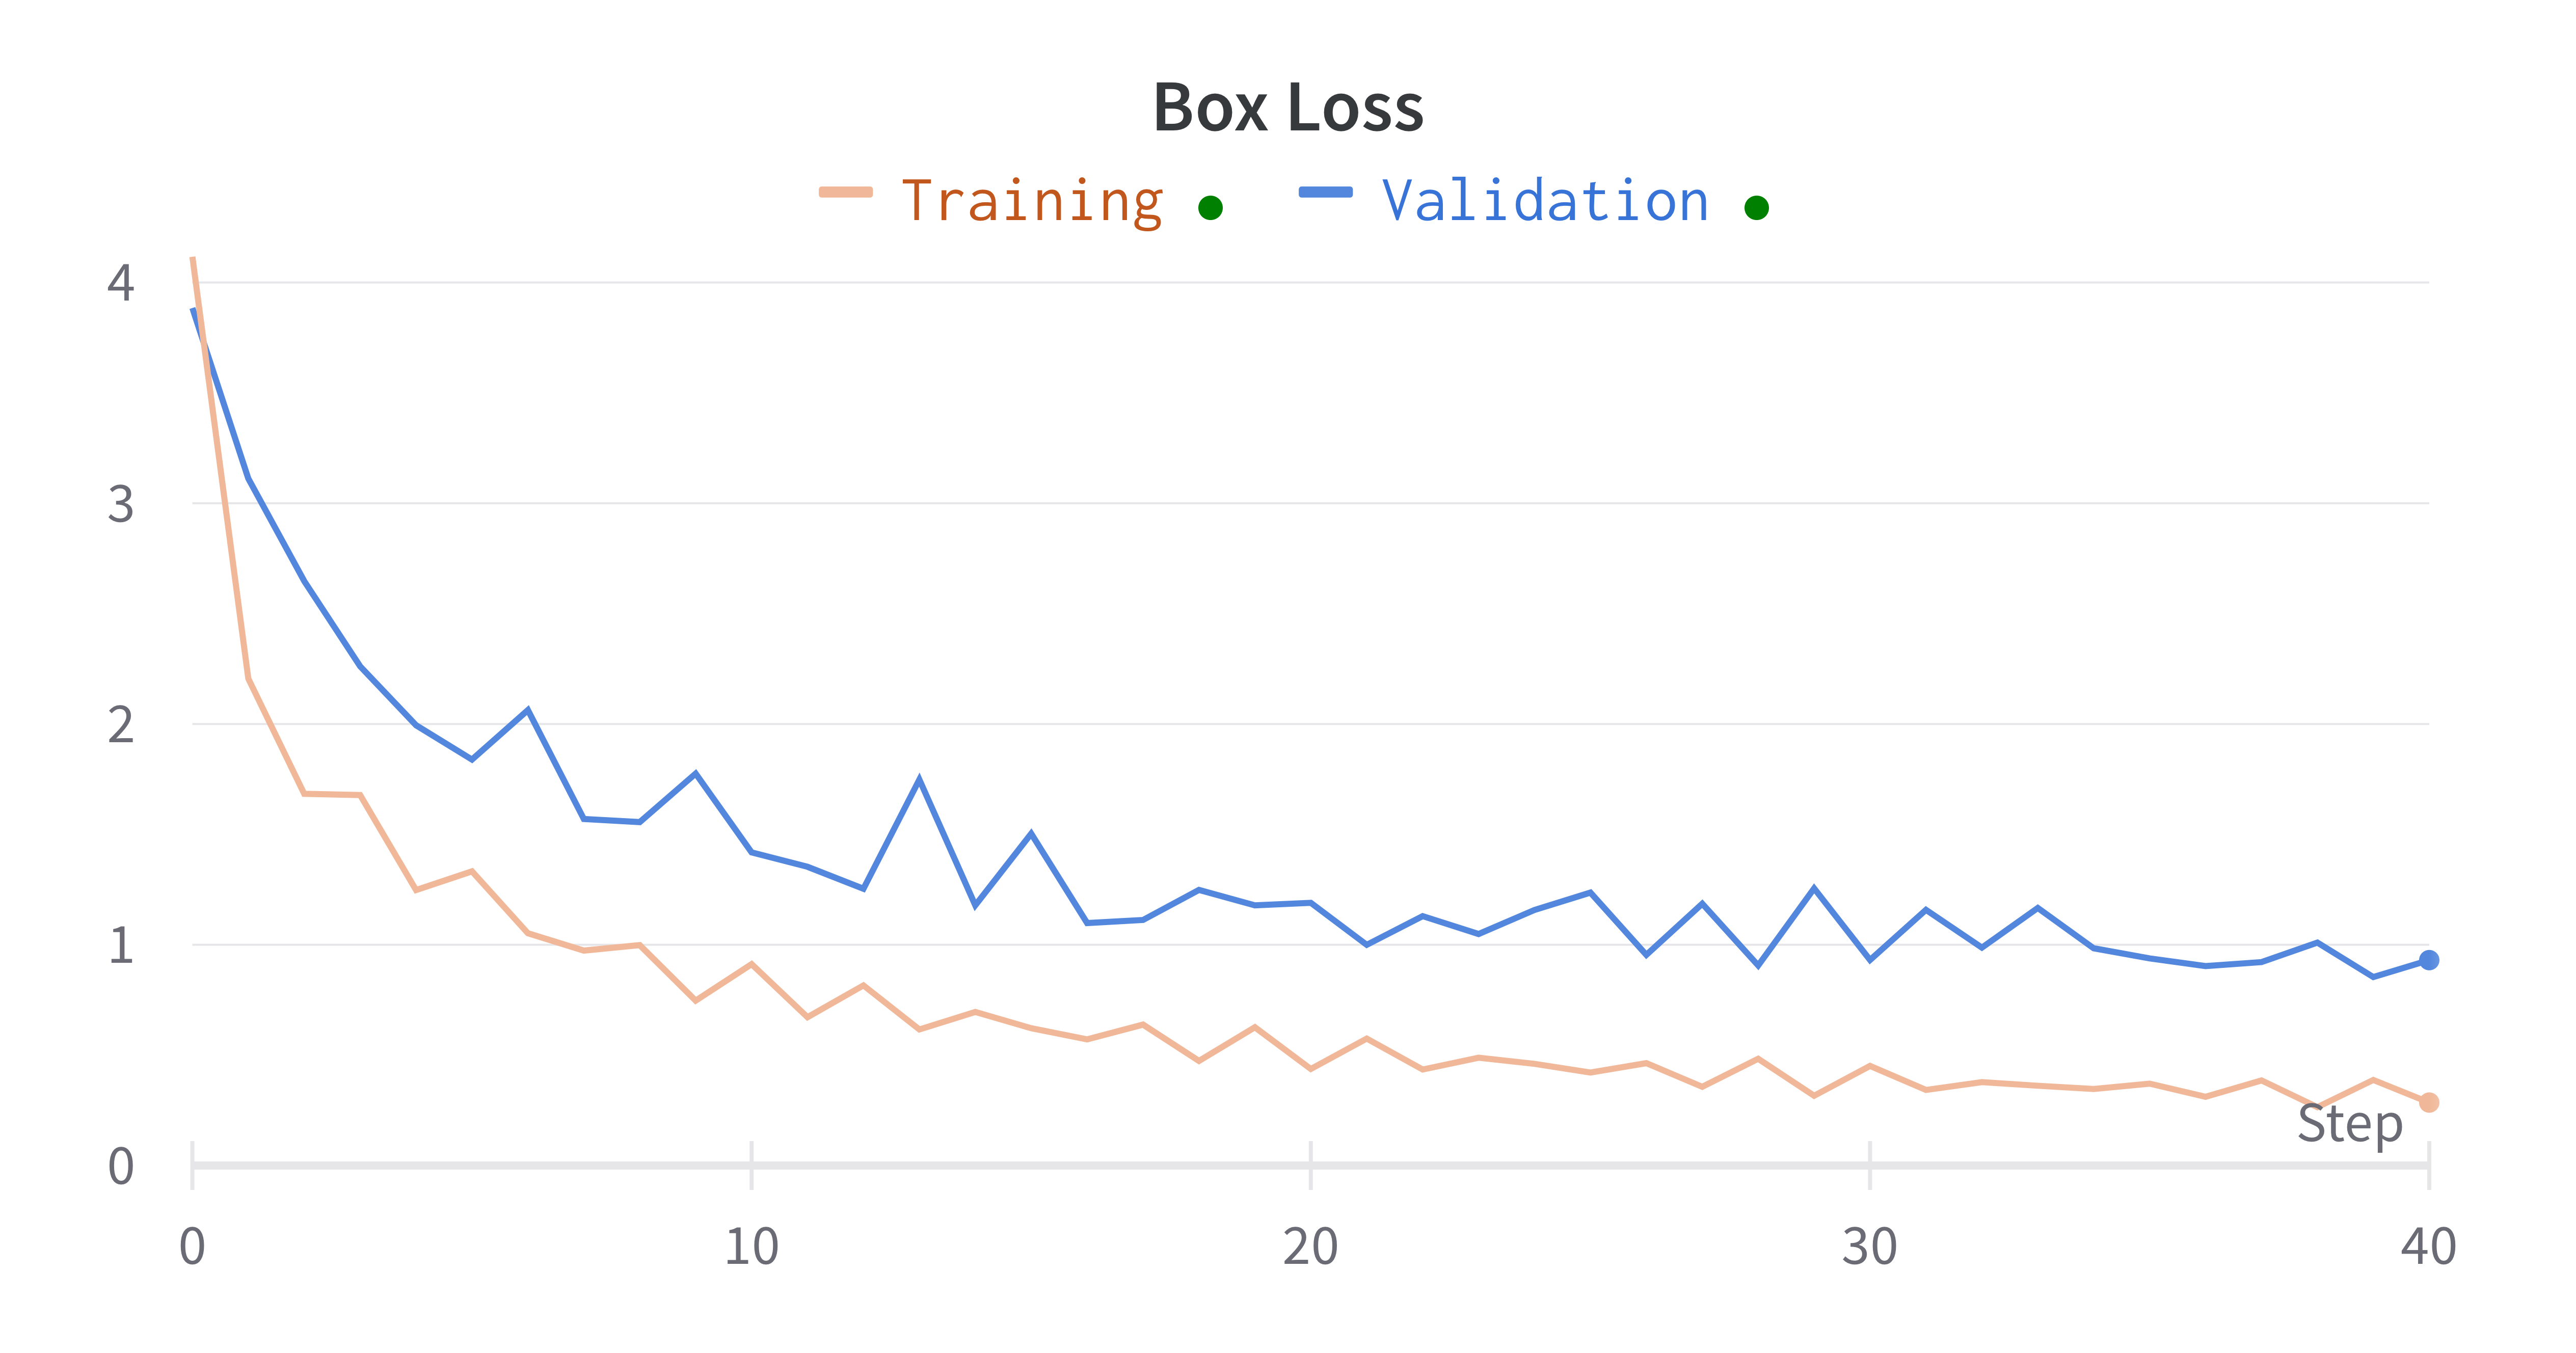
\includegraphics[width=\textwidth]{box_loss.png}
    \end{minipage}
    \caption{Total Loss and Box sub-Loss} % :)
    \label{fig:results_loss}
\end{figure}

\begin{figure}
    \begin{minipage}{0.48\textwidth}
        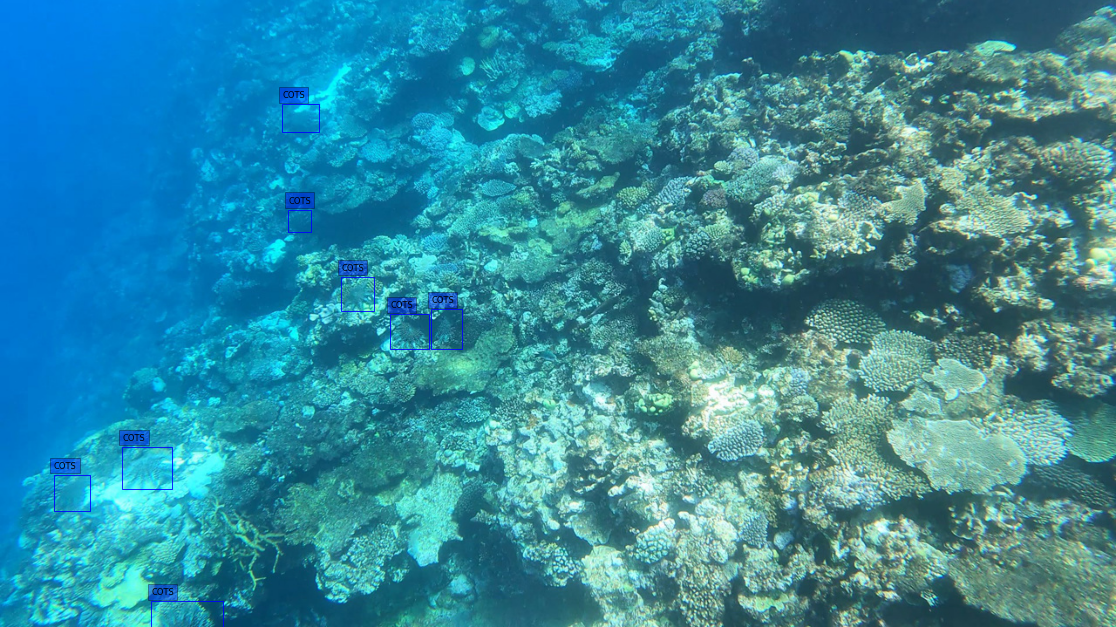
\includegraphics[width=\textwidth]{ground_truth.png}
    \end{minipage}
    \begin{minipage}{0.48\textwidth}
        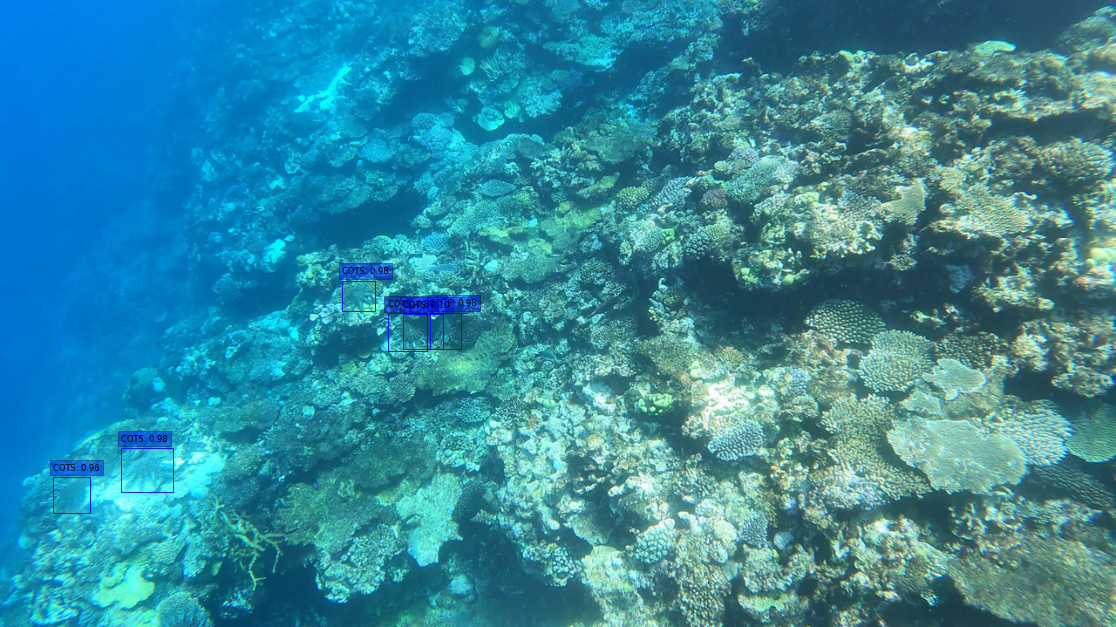
\includegraphics[width=\textwidth]{35.png}
    \end{minipage}
    \caption{Ground truth (left) and ReefNet predictions (right)}
    \label{fig:sample_visualizations}
\end{figure}


\begin{figure}
    \begin{minipage}{0.48\textwidth}
        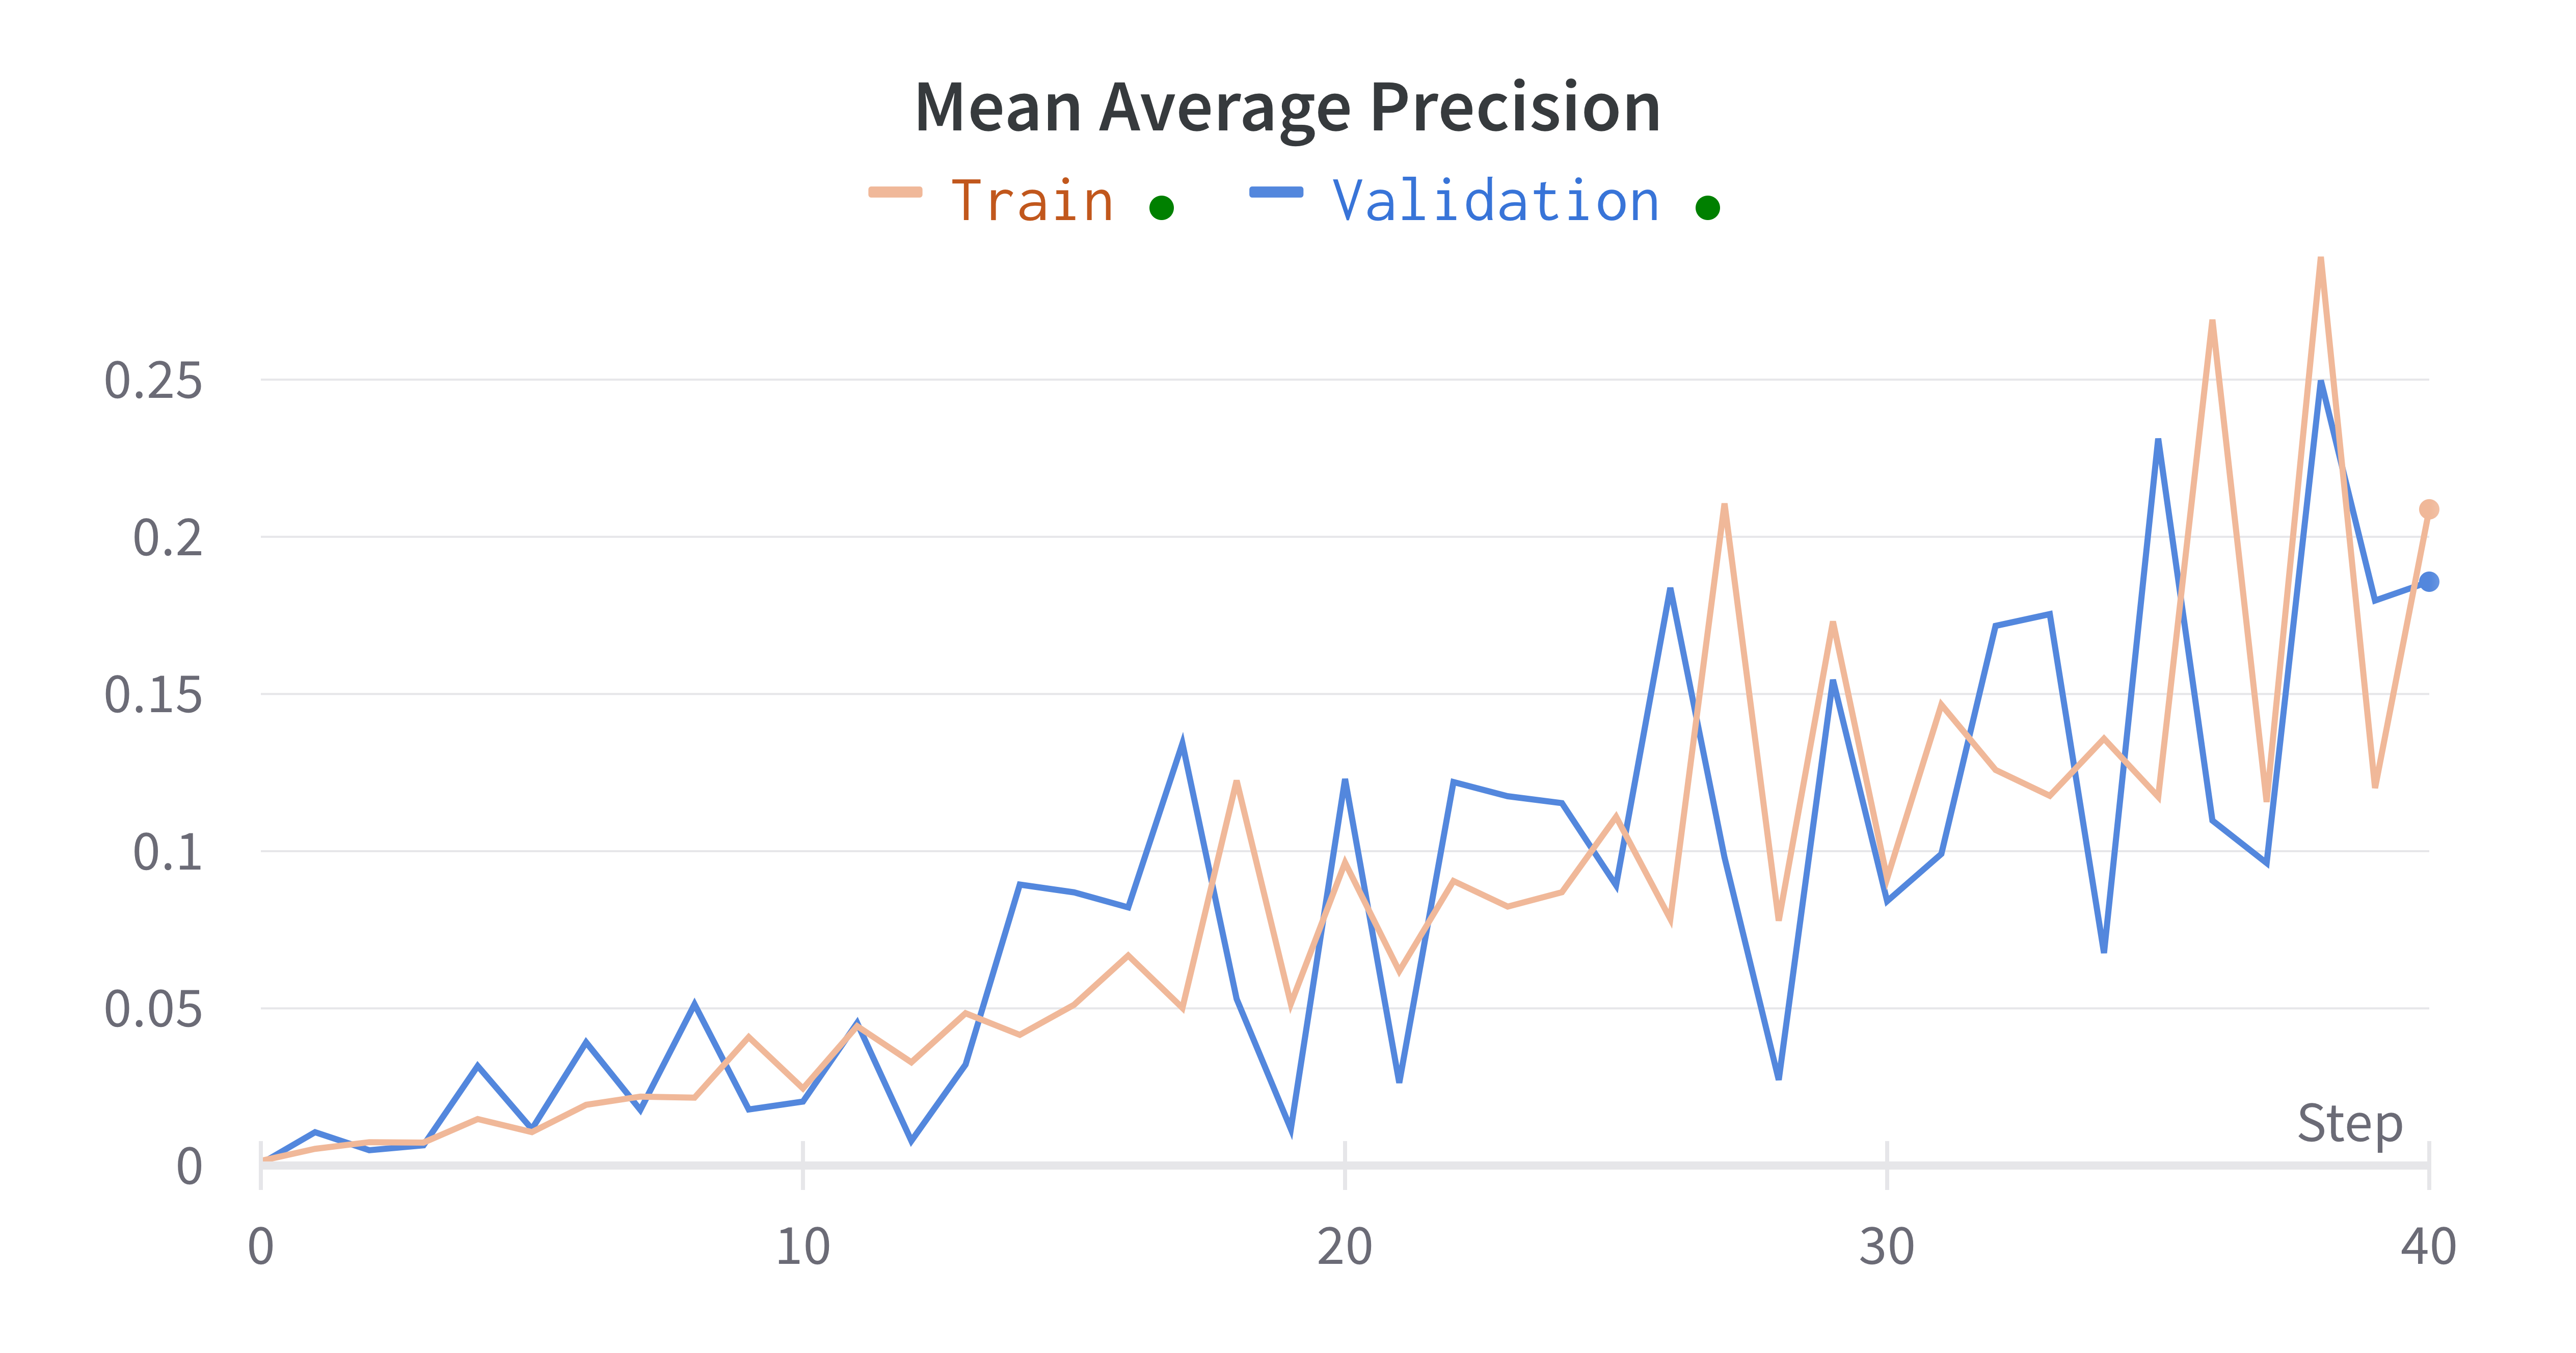
\includegraphics[width=\textwidth]{mean_average_precision_chart.png}
    \end{minipage}
    \begin{minipage}{0.48\textwidth}
        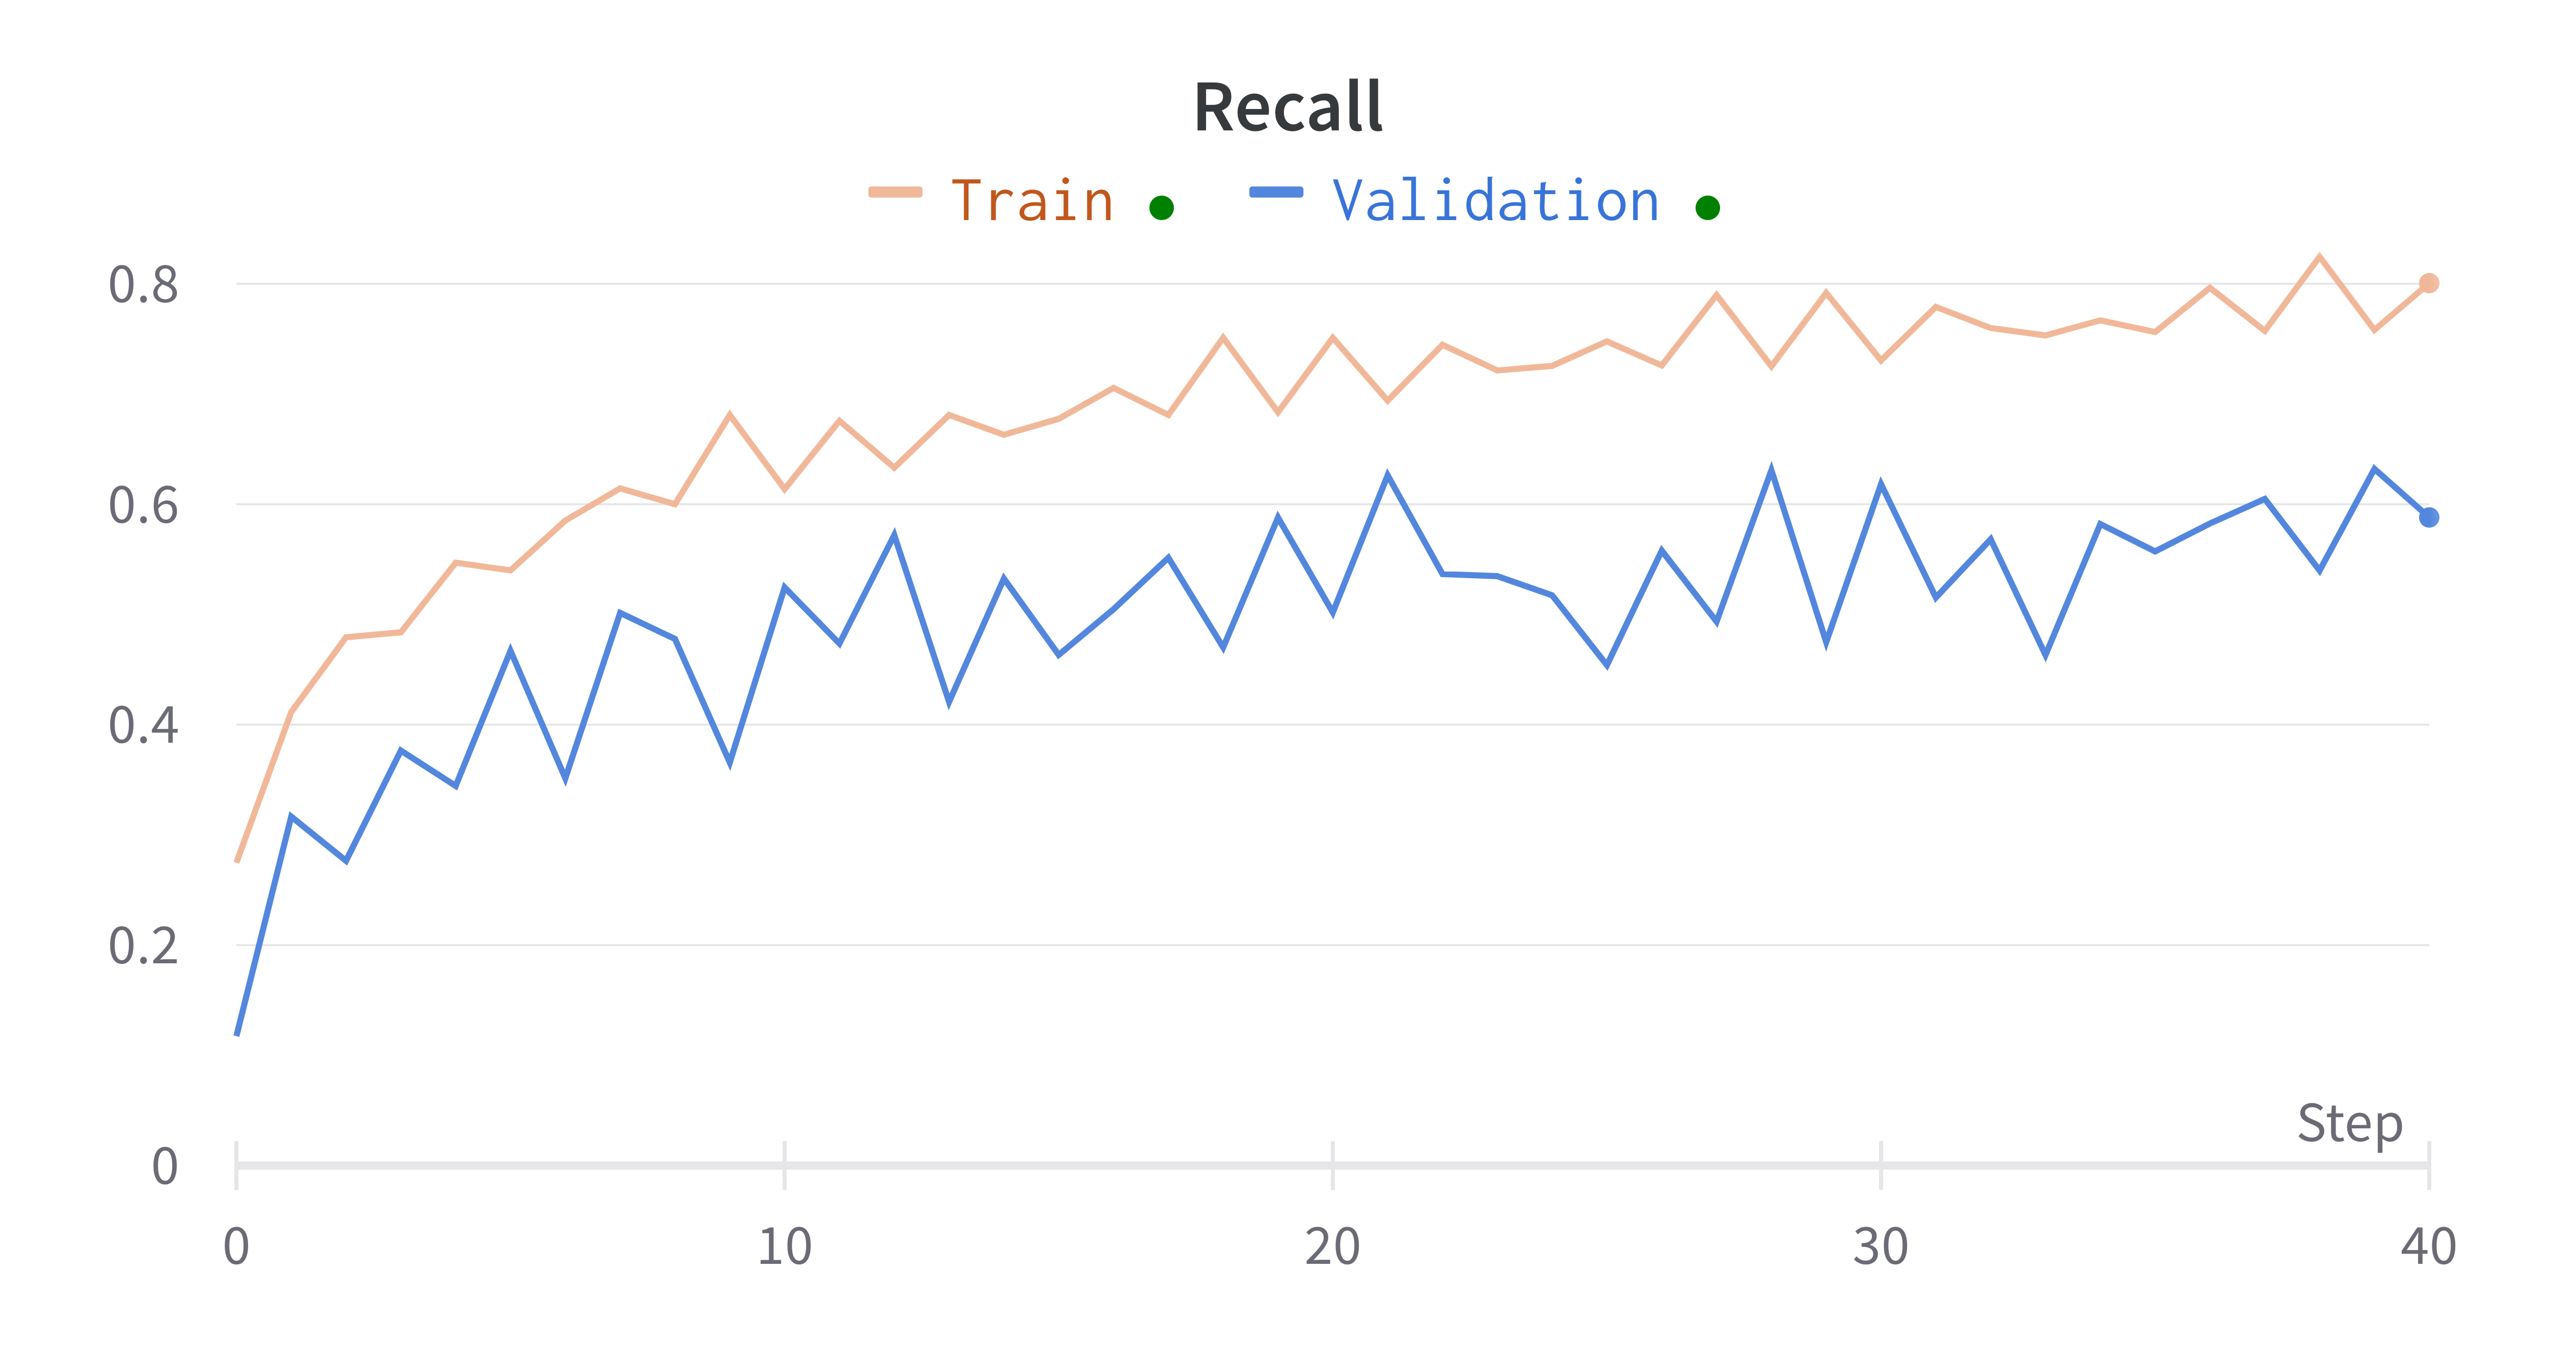
\includegraphics[width=\textwidth]{recall_chart.png}
    \end{minipage}
    \caption{MSCOCO Evaluation Metrics}
    \label{fig:metrics_eval}
\end{figure}



\section{Conclusions and Next Steps}
Despite achieving a low loss and strong Recall, ReefNet does not currently achieve strong Mean Average Precision.
Them model also converges on a substantially higher validation loss than training loss, as seen in Figure \ref{fig:results_loss}.
These factors both indicate that ReefNet is likely suffering from overfitting.
Although our data set includes 23k images, only 4k of those contain starfish and all of the images were generated from three continuous videos. 

This implies several issues: particular starfish present in these videos consistently show up in the same region of the video, all frames from one video have the same lighting conditions and hence same color distribution, and overall training data is extremely limited.
In order to remedy these issues, a good future step would be to introduce stronger data augmentation techniques.
Based on the results we have observed, we recommend the following specific augmentation techniques:

\textbf{Mosaic Augmentation.} The Mosaic augmentation, first proposed in the YOLOv4 paper \cite{yolov4}, simply cuts out different pieces of training images and meshes them together. In the case of our data set, this will be incredibly powerful as it will allow us to re-use starfish that only appear in a specific region of images and apply them across all training images.

\textbf{RandAugment.} RandAugment is a data augmentation technique consisting of both spatial and color distortions \cite{randaugment}. It corrupts images in various ways, producing numerous similar images from a single image.  During train time, RandAugment samples $n$ operations the list of color and spatial distortions.  Following this, it samples magnitudes from a normal distribution for use with each of these operations.  The way magnitude is used is specified on a per-operation basis; for example, in the Shear X operation the magnitude is used to determine how aggressively the image should be sheared.
By distorting training images using RandAugment, the resulting model tends to be more performant on images not included in the original training set.  

\textbf{CutMix.} CutMix is a regional dropout strategy \cite{cutmix}. CutMix simply cuts a rectangle from one image and overlays it onto a target image. Any bounding box labels present from within the CutOut section are used in the resulting image's detection targets. CutMix forces classifiers to become more strongly localized. Similar to Mosaic augmentation, this will allow us to remedy the issue of starfish only showing up in a limited number of locations in our training data set.

\textbf{MixUp.} MixUp is a technique to mitigate against overfitting and memorization. MixUp blends the pixel values between two images into a single resulting image. This forces models to favor simple linear behavior in between training examples \cite{mixup}. In the case of bounding box detection, MixUp simply uses the labels for both images as its prediction targets. Keras already offers a MixUp implementation with bounding box support \cite{wood2022kerascv}. 

\textbf{Closing Thoughts.} In this work we contribute a custom RetinaNet model written in Keras. In order to combat gradient explosion and numerical overflow we implement global norm gradient clipping. To further improve visibility into the learning process, we provide prediction visualization Keras callbacks. Our model has sophisticated metric tracking achieved through the use of Keras train\_step overriding.  Our training script integrates with Weights and Biases as well as TensorBoard to produce interactive metric dashboards.

Our model performs poorly when trained with the Adam optimizer \cite{adamoptimizer}, converging on a relatively high loss. On the other hand, training with the SGD optimizer \cite{ruder2016overview} yields strong results, with the model converging on a near-zero loss.

Our model has issues scoring a high Mean Average Precision.
This is likely due to the small volume of training data and lack of data augmentation techniques present in our pipeline.
This claim is supported by figure \ref{fig:results_loss}, which shows a massive discrepency between training and validation loss.
Follow up works should implement data augmentation techniques such as the Mosaic Augmentation, RandAugment, CutMix, and MixUp.
Combining these augmentations will produce a more robust version of ReefNet.

\printbibliography
\end{document}